\documentclass[conference]{IEEEtran}
\IEEEoverridecommandlockouts
\usepackage{cite}
\usepackage{float}
\usepackage{amsmath,amssymb,amsfonts}
\usepackage{graphicx}
\usepackage{textcomp}
\usepackage{xcolor}
\usepackage[utf8]{inputenc}
\usepackage[T1]{fontenc}
\usepackage[portuguese]{babel}
\usepackage{booktabs}
\usepackage[export]{adjustbox}

\begin{document}

\title{Análise de Desempenho de Técnicas de Aprendizagem Automática para Previsão da Capacidade de Postos de Transformação no Contexto da Mobilidade Elétrica}

\author{
\IEEEauthorblockN{Rui Santiago}
\IEEEauthorblockA{\textit{Dept. de Engenharia Informática} \\
\textit{ISEP} \\ Porto, Portugal \\ 1221402@isep.ipp.pt}
\and
\IEEEauthorblockN{Rui Silva}
\IEEEauthorblockA{\textit{Dept. de Engenharia Informática} \\
\textit{ISEP} \\ Porto, Portugal \\ 1231105@isep.ipp.pt}
\and
\IEEEauthorblockN{Tiago Barros}
\IEEEauthorblockA{\textit{Dept. de Engenharia Informática} \\
\textit{ISEP} \\ Porto, Portugal \\ 1231108@isep.ipp.pt}
}

\maketitle

% -------------------------------------------------------------------
\begin{abstract}
A transição energética europeia impõe uma pressão crescente sobre a infraestrutura elétrica municipal, nomeadamente nos Postos de Transformação de Distribuição (PTD), que constituem o elo entre a rede de média tensão e os consumidores finais. Este trabalho analisa, ao nível do PTD, o impacto da substituição de iluminação pública convencional por tecnologia LED na folga de potência disponível, avaliando a viabilidade técnica de realocar essa capacidade para infraestruturas de carregamento de veículos elétricos. Foram aplicadas técnicas de aprendizagem automática, nomeadamente regressão linear múltipla, árvores de decisão, SVM e redes neuronais, para a previsão contínua da folga de potência por PTD e para a classificação do nível de ocupação da rede. A avaliação foi conduzida com validação cruzada k-fold e os resultados comparados com testes de significância estatística. Para a regressão, a rede neuronal alcançou o melhor desempenho (MAE de 35,42 kVA), com diferença estatisticamente significativa face à árvore de decisão (p < 0,05). Para a classificação, a rede neuronal também se destacou com uma accuracy de 67,85\% e F1-score de 0,6623, superando os restantes modelos. Os resultados evidenciam que o perfil construtivo do PTD e a capacidade instalada são os preditores mais relevantes, e que a classe média de ocupação representa o principal desafio de generalização para todos os modelos testados.
\end{abstract}

\begin{IEEEkeywords}
aprendizagem automática, postos de transformação, folga de potência, mobilidade elétrica, iluminação pública LED, redes neuronais, SVM, classificação, regressão
\end{IEEEkeywords}

% -------------------------------------------------------------------
\section{Introdução}

A descarbonização das cidades europeias impõe uma dupla pressão sobre a rede elétrica de baixa tensão: por um lado, a substituição massiva de iluminação pública por tecnologia LED reduz significativamente a carga nos PTD; por outro, a expansão acelerada da mobilidade elétrica exige potência disponível nos mesmos pontos de transformação \cite{eredes}. Esta sinergia potencial constitui o núcleo do desafio proposto pela e-REDES: quantificar a capacidade libertada pela eficiência energética na iluminação e determinar se essa capacidade é suficiente para suportar infraestruturas de carregamento de veículos elétricos (VE), sem comprometer a estabilidade da rede.

O presente trabalho corresponde à segunda iteração do Trabalho Prático da unidade curricular de Análise de Dados em Informática, evoluindo de uma análise exploratória ao nível do concelho (TP1) para uma modelação preditiva ao nível do PTD. O \textit{dataset} utilizado agrega dados de iluminação pública e de postos de transformação para cerca de 72\,000 PTDs distribuídos por Portugal continental.

Os objetivos específicos são: (i) realizar uma análise exploratória dos dados ao nível do PTD; (ii) desenvolver e comparar modelos de regressão para prever a folga de potência ($P_{Folga\_PTD}$); (iii) desenvolver e comparar modelos de classificação para o nível de ocupação da rede (\textit{utilizRede}); e (iv) selecionar, com suporte estatístico, o modelo com melhor desempenho em cada tarefa.

% -------------------------------------------------------------------
\section{Estado da Arte}

A análise de desempenho de técnicas de aprendizagem automática aplicadas a redes elétricas de distribuição tem sido alvo de crescente atenção. Abordagens baseadas em redes neuronais artificiais e SVM demonstraram capacidade superior na previsão de carga em transformadores de distribuição comparativamente a modelos lineares clássicos \cite{bishop2006,mitchell1997}. A integração de variáveis de iluminação pública e de perfis de consumo ao nível do PTD é, contudo, uma abordagem relativamente recente, impulsionada pela disponibilização de dados operacionais por parte das distribuidoras de energia.

\subsection{Regressão}
A \textbf{regressão linear múltipla} constitui uma base interpretável para modelação de variáveis contínuas, com a limitação de assumir linearidade entre preditores e resposta \cite{mitchell1997}. As \textbf{árvores de regressão} superam esta limitação ao capturar não-linearidades, mas são propensas a \textit{overfitting} sem poda adequada. O \textbf{SVM} para regressão (SVR) com kernel RBF demonstra bom desempenho em dados com relações não-lineares complexas \cite{bishop2006}. As \textbf{redes neuronais} com regularização e \textit{early stopping} têm mostrado resultados competitivos em previsão de carga, desde que devidamente otimizadas.

\subsection{Classificação}
Para classificação multiclasse, \textbf{árvores de decisão} oferecem interpretabilidade e identificação de variáveis relevantes. O \textbf{KNN} é sensível à escala dos dados e ao parâmetro $k$. O \textbf{SVM} multiclasse (OvR) apresenta bom desempenho em espaços de alta dimensão, mas pode sofrer com desequilíbrio de classes. As \textbf{redes neuronais} permitem maior capacidade expressiva, a custo de maior complexidade de otimização \cite{bishop2006}.

% -------------------------------------------------------------------
\section{Metodologia}

\subsection{Dataset e Variáveis}

O \textit{dataset} PTD\_level\_dataset.xlsx resulta da junção de dados de iluminação pública (IP\_data.xlsx) e de postos de transformação (PTD\_data.xlsx), pela variável \textit{CodDistritoConcelho}. Contém aproximadamente 72\,000 registos com as variáveis descritas na Tabela~\ref{tab:variaveis}.

\begin{table}[htbp]
\caption{Variáveis do Dataset}
\label{tab:variaveis}
\begin{center}
\begin{tabular}{lll}
\toprule
\textbf{Nível PTD} & \textbf{Agregadas Concelho} & \textbf{Derivadas} \\
\midrule
Cap\_PTD\_kVA & P\_IP\_Total & PFolga\_PTD \\
N\_Clientes & Rate\_Ineficiencia & Cap\_per\_Cliente \\
Pot\_Contratada\_kVA & LED\_Ratio & IP\_per\_PTD \\
Tipo\_Construtivo & & $\Delta P_{LED}$, $D$ \\
\bottomrule
\end{tabular}
\end{center}
\end{table}

As variáveis derivadas calculadas incluem o Ganho LED ($\Delta P_{LED}$), a Folga Rede ($P_{Folga}$), a Carga VE ($P_{VE}$) e o Saldo Final de Viabilidade ($D$). A variável \textit{utilizRede} foi obtida por discretização de \textit{Util\_Decimal} em três classes (baixo, médio, alto) com base em quantis, garantindo distribuição equilibrada entre classes.

\subsection{Pré-processamento}

O pré-processamento incluiu: (i) remoção de registos com valores omissos nas variáveis-alvo; (ii) codificação \textit{one-hot} de \textit{Tipo\_Construtivo}; (iii) normalização Min-Max para SVM e redes neuronais; (iv) seleção de variáveis por correlação de Pearson com $P_{Folga\_PTD}$ (Fig.~\ref{fig:correlacao}) e por importância em árvores de decisão. Variáveis com correlação próxima de zero ou com elevada colinearidade foram excluídas.

\begin{figure}[htbp]
\centerline{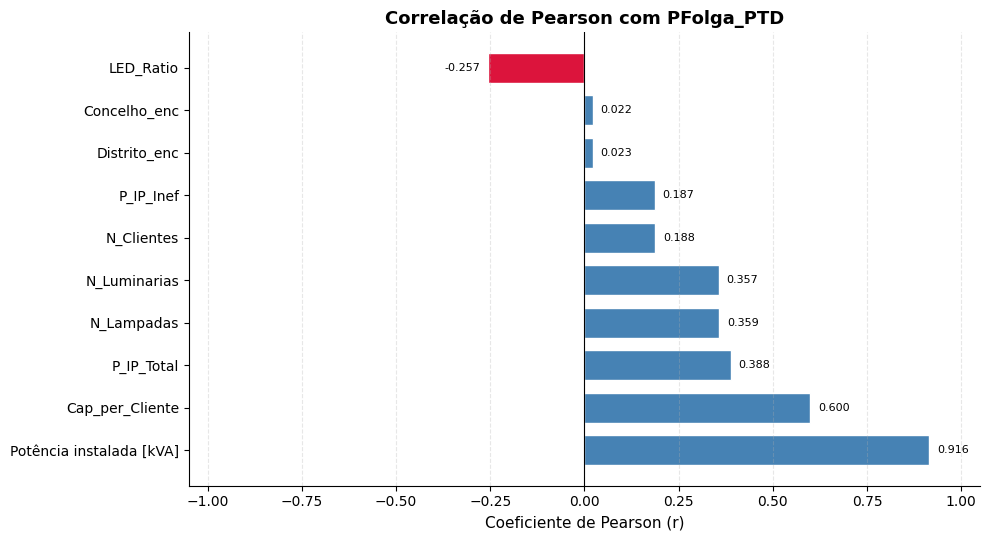
\includegraphics[width=\columnwidth]{./img/correlacao_de_pearson_folga.png}}
\caption{Correlação de Pearson entre $P_{Folga\_PTD}$ e as restantes variáveis.}
\label{fig:correlacao}
\end{figure}

\subsection{Protocolo de Avaliação}

Todos os modelos foram avaliados com validação cruzada k-fold ($k=10$), reportando média e desvio padrão das métricas. Para regressão utilizaram-se MAE e RMSE; para classificação, Accuracy, Precision, Recall e F1-score (macro e por classe). A significância estatística das diferenças entre os dois melhores modelos foi verificada com o t-test pareado ($\alpha = 0.05$), após confirmação de normalidade das distribuições de erro.

% -------------------------------------------------------------------
\section{Análise Exploratória de Dados}

A Fig.~\ref{fig:distribuicao} apresenta a distribuição das principais variáveis. A variável $P_{Folga\_PTD}$ exibe assimetria positiva com cauda longa, sugerindo a presença de PTDs com folga muito elevada (tipicamente zonas rurais com baixa densidade de consumo). A variável \textit{Util\_Decimal} concentra-se entre 0,2 e 0,6, com a classe médio a ser a mais representada após discretização por quantis.

\begin{figure}[htbp]
\centerline{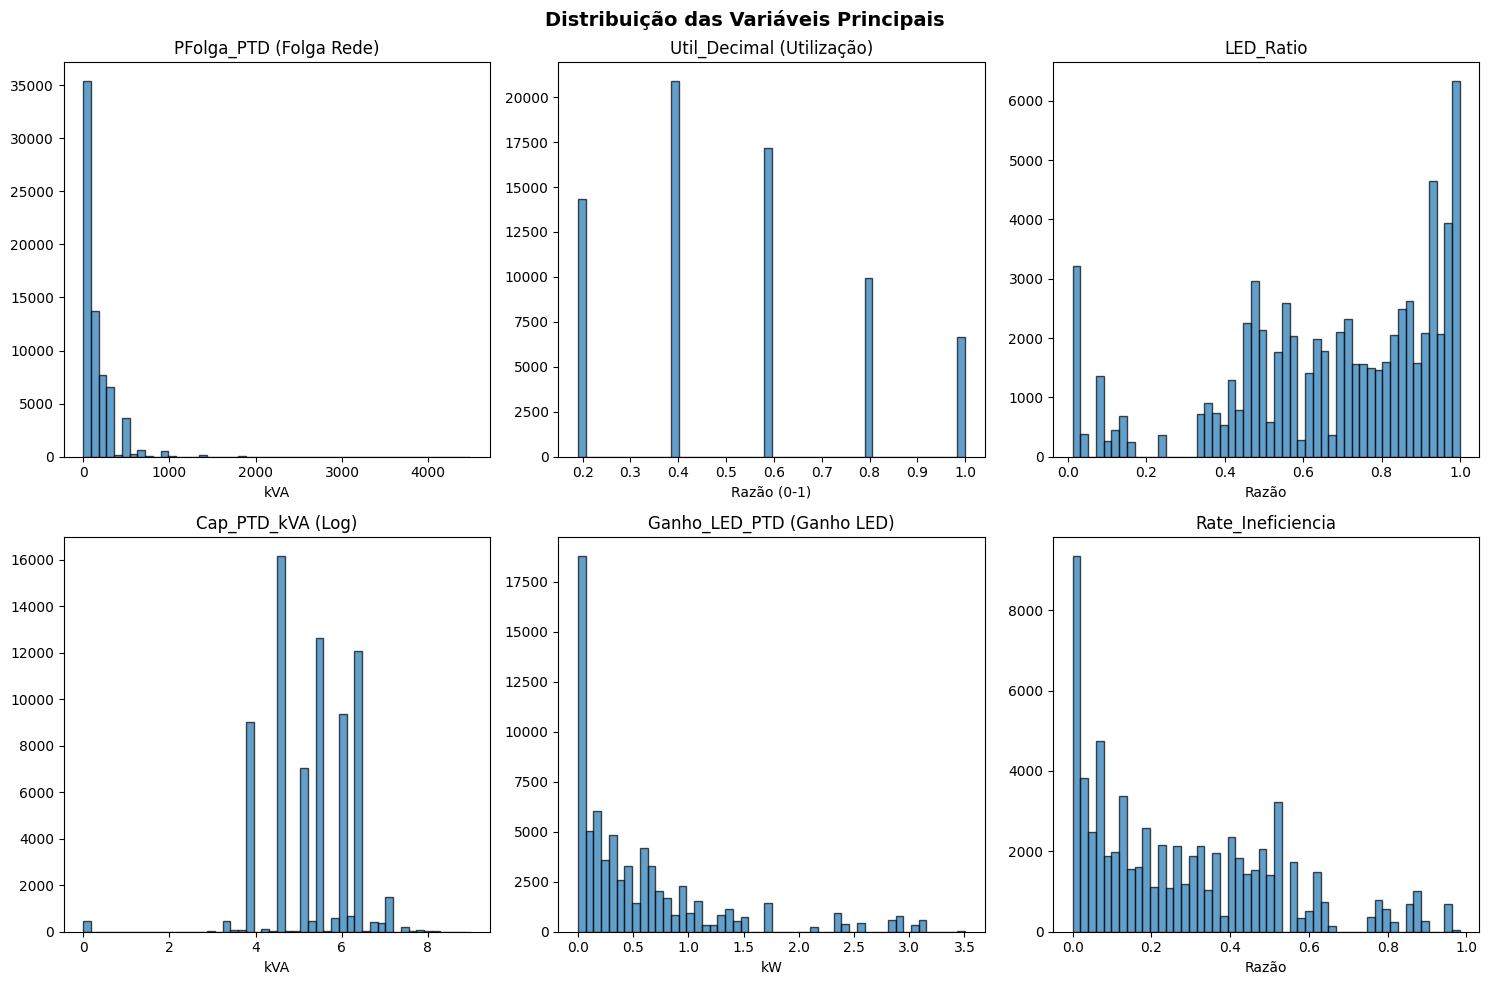
\includegraphics[width=\columnwidth]{./img/distribuicao_variaveis.png}}
\caption{Distribuição das principais variáveis do \textit{dataset}.}
\label{fig:distribuicao}
\end{figure}

A análise por distrito (Fig.~\ref{fig:distrito}) revela heterogeneidade geográfica significativa: distritos do interior apresentam PTDs com folgas médias superiores, enquanto Lisboa e Porto concentram PTDs com ocupação mais próxima do limite operacional.

\begin{figure}[htbp]
\centerline{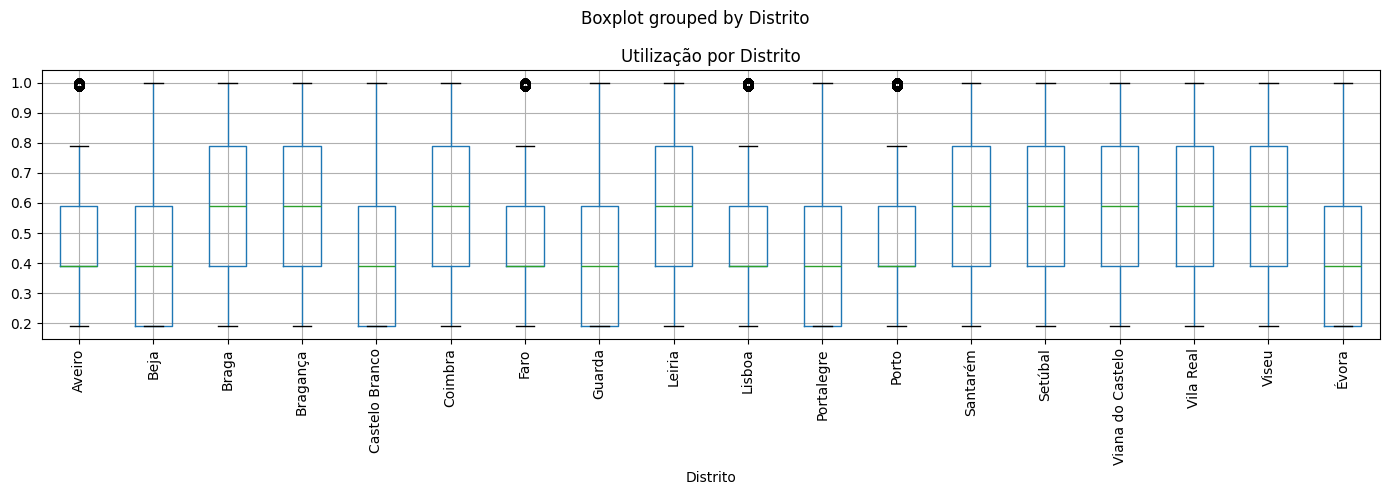
\includegraphics[width=\columnwidth]{./img/utilizacao_distrito.png}}
\caption{Utilização da rede por distrito.}
\label{fig:distrito}
\end{figure}

A matriz de correlação completa (Fig.~\ref{fig:corr_dataset}) confirma que \textit{Cap\_PTD\_kVA} e \textit{Pot\_Contratada\_kVA} são os preditores mais correlacionados com $P_{Folga\_PTD}$, enquanto variáveis de iluminação pública (\textit{LED\_Ratio}, \textit{P\_IP\_Total}) apresentam correlação moderada, justificando a sua inclusão nos modelos mas não como preditores exclusivos.

\begin{figure}[htbp]
\centerline{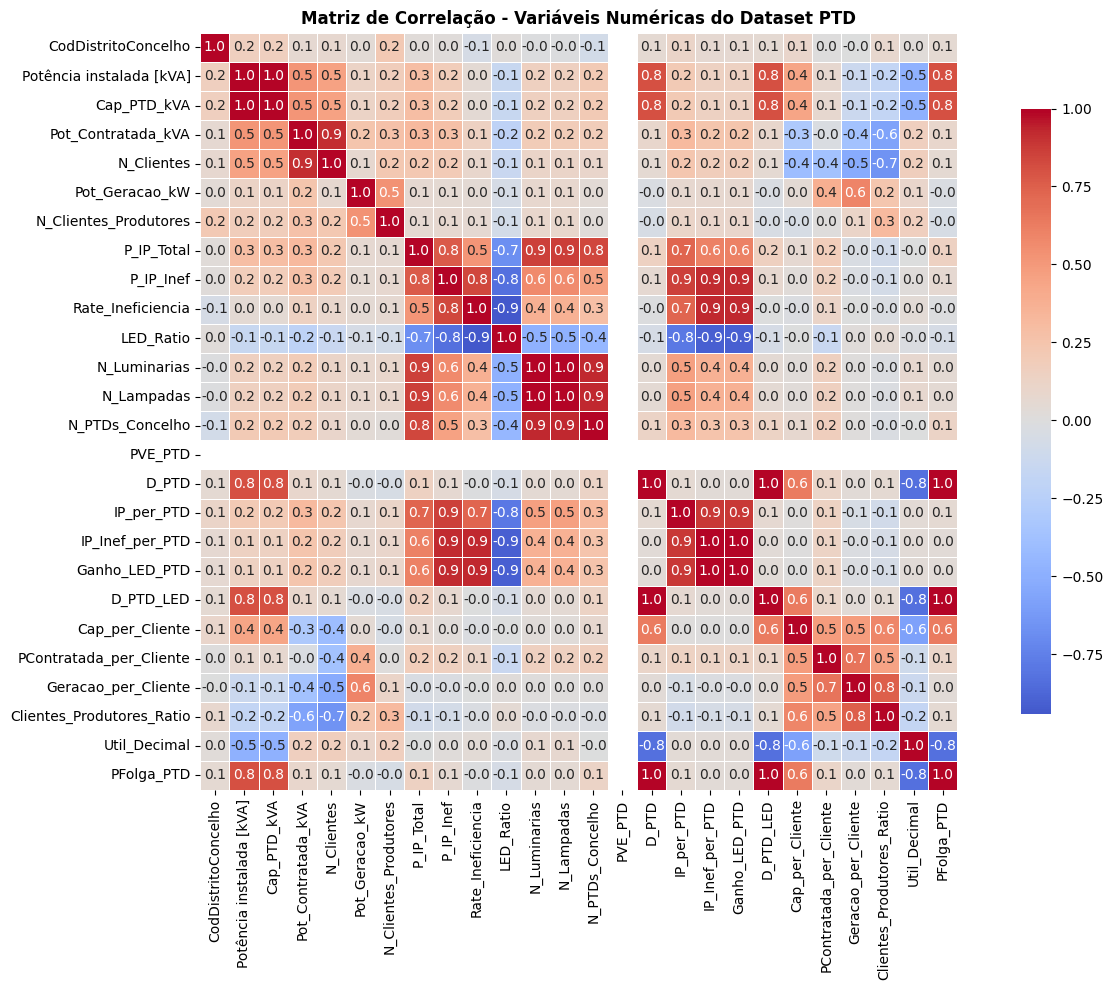
\includegraphics[width=\columnwidth]{./img/correlacao_dataset.png}}
\caption{Matriz de correlação do \textit{dataset}.}
\label{fig:corr_dataset}
\end{figure}

% -------------------------------------------------------------------
\section{Regressão: Previsão de $P_{Folga\_PTD}$}

\subsection{Regressão Linear Simples}

Como variável explicativa para a regressão linear simples foi selecionada \textit{Cap\_PTD\_kVA}, por apresentar a correlação de Pearson mais elevada com $P_{Folga\_PTD}$ (Fig.~\ref{fig:correlacao}). A Fig.~\ref{fig:reg_linear} ilustra a reta ajustada e o diagrama de dispersão correspondente.

\begin{figure}[htbp]
\centerline{
\includegraphics[width=\columnwidth]{./img/pesado/regressao_linear_simples.png}}
\caption{Regressão linear simples: $P_{Folga\_PTD}$ em função de \textit{Cap\_PTD\_kVA}.}
\label{fig:reg_linear}
\end{figure}

\subsection{Modelos Múltiplos}

Foram desenvolvidos quatro modelos com k-fold ($k=10$): regressão linear múltipla, árvore de regressão, SVR (kernel RBF otimizado por grid search) e rede neuronal (configuração otimizada com duas camadas ocultas, regularização L2 e \textit{early stopping}). A Tabela~\ref{tab:regressao} resume os resultados.

\begin{table}[htbp]
\caption{Resultados de Regressão -- Perfil Pesado (k-fold, $k=10$)}
\label{tab:regressao}
\begin{center}
\begin{tabular}{lcccc}
\toprule
\textbf{Modelo} & \textbf{MAE} & \textbf{$\pm$} & \textbf{RMSE} & \textbf{$\pm$} \\
\midrule
Linear     & 37,50 & 0,47 & 57,31 & 1,25 \\
Tree       & 36,32 & 0,35 & 58,85 & 1,56 \\
SVM        & 36,72 & 0,41 & 59,38 & 1,35 \\
NeuralNet  & \textbf{35,42} & \textbf{0,45} & \textbf{55,35} & \textbf{1,63} \\
\bottomrule
\end{tabular}
\end{center}
\end{table}

A rede neuronal obteve o menor MAE (35,42 kVA) e RMSE (55,35 kVA). A Fig.~\ref{fig:comparacao_reg} compara visualmente os quatro modelos.

\begin{figure}[htbp]
\centerline{
\includegraphics[width=\columnwidth]{./img/pesado/comparacao_global.png}}
\caption{Comparação de modelos de regressão (MAE e RMSE).}
\label{fig:comparacao_reg}
\end{figure}

A Fig.~\ref{fig:arvore_reg} apresenta a árvore de regressão obtida. As divisões de topo confirmam \textit{Cap\_PTD\_kVA} e \textit{Pot\_Contratada\_kVA} como os preditores dominantes, consistente com a análise de correlação.

\begin{figure}[htbp]
\centerline{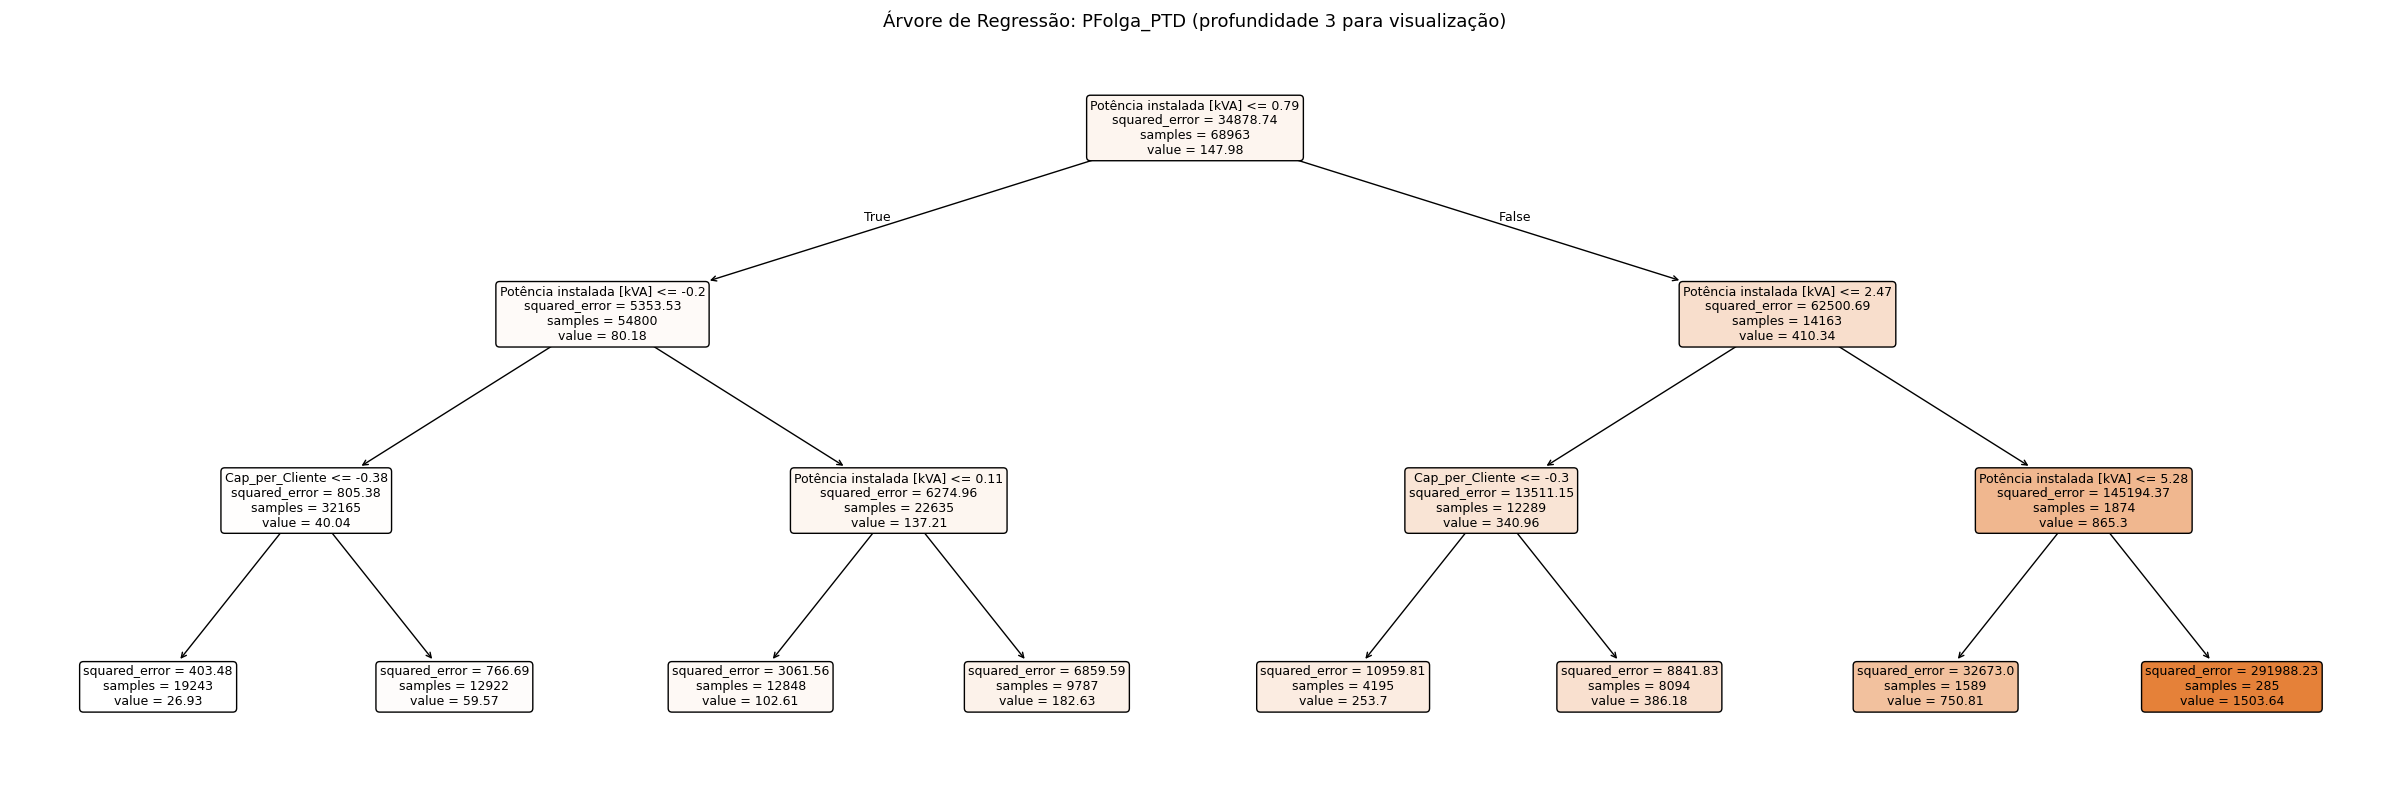
\includegraphics[width=\columnwidth]{./img/pesado/arvore_regressao.png}}
\caption{Árvore de regressão para $P_{Folga\_PTD}$.}
\label{fig:arvore_reg}
\end{figure}

\subsection{Curvas de Aprendizagem}

As curvas de aprendizagem para os dois melhores modelos (NeuralNet e Tree) são apresentadas na Fig.~\ref{fig:curvas_reg}. A rede neuronal apresenta convergência das curvas de treino e validação, com gap de apenas 0,40 kVA (MAE treino: 34,89; validação: 35,30), indicando treino adequado sem \textit{overfitting} relevante. A árvore de decisão apresenta um gap superior (3,95 kVA), sugestivo de ligeiro \textit{overfitting}.

\begin{figure}[htbp]
\centerline{
\includegraphics[width=\columnwidth]{./img/pesado/curvas_aprendizagem_regressao.png}}
\caption{Curvas de aprendizagem -- NeuralNet e Tree (regressão).}
\label{fig:curvas_reg}
\end{figure}

\subsection{Teste de Significância Estatística}

Aplicou-se o t-test pareado entre NeuralNet e Decision Tree. Ambas as distribuições de erro por fold são normais (confirmado pelo teste de Shapiro-Wilk), justificando o uso de teste paramétrico. O resultado ($t = 11,79$; $p < 0,0001$) confirma que a diferença é estatisticamente significativa ($\alpha = 0.05$). O modelo NeuralNet é o melhor modelo de regressão.

% -------------------------------------------------------------------
\section{Classificação: Previsão de \textit{utilizRede}}

\subsection{Definição das Classes}

A variável \textit{utilizRede} foi derivada de \textit{Util\_Decimal} por discretização em quantis ($Q_{33}$ e $Q_{67}$), originando três classes equilibradas: \textbf{baixo} ($< Q_{33}$), \textbf{médio} ($Q_{33}$--$Q_{67}$) e \textbf{alto} ($> Q_{67}$). Esta abordagem foi preferida a intervalos fixos por garantir maior equilíbrio entre classes, reduzindo o viés dos classificadores para a classe maioritária.

\subsection{Modelos e Resultados Globais}

Foram desenvolvidos quatro modelos: árvore de decisão, rede neuronal (otimizada), SVM (kernel RBF) e KNN (k otimizado por grid search). A Tabela~\ref{tab:classificacao} resume as métricas globais.

\begin{table}[htbp]
\caption{Resultados de Classificação -- Perfil Pesado (k-fold, $k=10$)}
\label{tab:classificacao}
\begin{center}
\begin{tabular}{lcccc}
\toprule
\textbf{Modelo} & \textbf{Acc} & \textbf{Prec} & \textbf{Rec} & \textbf{F1} \\
\midrule
Decision Tree & 0,6605 & 0,6400 & 0,6605 & 0,6443 \\
\textbf{NeuralNet}  & \textbf{0,6785} & \textbf{0,6609} & \textbf{0,6785} & \textbf{0,6623} \\
SVM           & 0,6220 & 0,5959 & 0,6220 & 0,5398 \\
KNN           & 0,6605 & 0,6359 & 0,6605 & 0,6401 \\
\bottomrule
\end{tabular}
\end{center}
\end{table}

A rede neuronal superou todos os modelos em todas as métricas globais. O SVM revelou o pior desempenho, com F1-score de apenas 0,54, penalizado em particular na classe \textit{médio}.

\subsection{Desempenho por Classe}

A Fig.~\ref{fig:f1_classe} ilustra o F1-score por classe para cada modelo. A classe \textbf{baixo} é a mais fácil de classificar (F1 $\approx$ 0,80 para NeuralNet), ao passo que a classe \textbf{médio} apresenta os piores resultados em todos os modelos (F1 $\approx$ 0,41 para NeuralNet). Este padrão é consistente com a maior sobreposição de distribuições para a classe intermédia, um fenómeno esperado em discretizações baseadas em quantis.

\begin{figure}[htbp]
\centerline{
\includegraphics[width=\columnwidth]{./img/pesado/f1score_por_classe_modelo.png}}
\caption{F1-score por classe e por modelo (classificação).}
\label{fig:f1_classe}
\end{figure}

A Fig.~\ref{fig:conf_matrix} apresenta a matriz de confusão do melhor modelo (NeuralNet). Confirma-se que os erros mais frequentes ocorrem na fronteira entre as classes \textit{médio} e \textit{alto}, e entre \textit{médio} e \textit{baixo}.

\begin{figure}[htbp]
\centerline{
\includegraphics[width=\columnwidth]{./img/pesado/matriz_de_confusao.png}}
\caption{Matriz de confusão -- NeuralNet (classificação).}
\label{fig:conf_matrix}
\end{figure}

\subsection{Importância de Variáveis}

A Fig.~\ref{fig:feat_imp} compara a importância de variáveis na árvore de decisão com as correlações de Pearson identificadas na análise exploratória. \textit{Cap\_PTD\_kVA} e \textit{Pot\_Contratada\_kVA} dominam ambas as perspetivas, validando a coerência entre a análise estatística e o modelo preditivo. As variáveis de iluminação pública têm importância secundária mas não negligenciável.

\begin{figure}[htbp]
\centerline{
\includegraphics[width=\columnwidth]{./img/pesado/importancia_feature_vs_correlacao_utilzRede.png}}
\caption{Importância de variáveis (árvore de decisão) vs. correlação de Pearson.}
\label{fig:feat_imp}
\end{figure}

\subsection{Curvas de Aprendizagem}

As curvas de aprendizagem do melhor (NeuralNet) e pior (SVM) modelo são apresentadas na Fig.~\ref{fig:curvas_class}. A NeuralNet apresenta curvas convergentes com gap negativo de $-0,009$ (F1 validação ligeiramente superior ao de treino), indicando treino adequado. O SVM apresenta convergência prematura com F1 baixo em ambas as curvas ($\approx 0,54$), sugestivo de \textit{underfitting}: o modelo não tem capacidade suficiente para capturar a complexidade dos padrões de ocupação da rede.

\begin{figure}[htbp]
\centerline{
\includegraphics[width=\columnwidth]{./img/pesado/curvas_aprendizagem_class.png}}
\caption{Curvas de aprendizagem -- NeuralNet e SVM (classificação).}
\label{fig:curvas_class}
\end{figure}

\subsection{Teste de Significância Estatística}

O t-test pareado entre NeuralNet e Decision Tree ($t = 11,79$; $p < 0,0001$) confirma diferença estatisticamente significativa no F1-score ($\alpha = 0.05$). O modelo NeuralNet é o melhor modelo de classificação.

% -------------------------------------------------------------------
\section{Discussão e Limitações}

Os resultados mostram que a rede neuronal é consistentemente superior nas duas tarefas, mas os ganhos absolutos sobre a árvore de decisão são modestos (MAE: $-0,90$ kVA; F1: $+0,018$), o que tem implicações práticas: em cenários de \textit{deployment} com restrições de interpretabilidade ou latência, a árvore de decisão pode ser uma alternativa razoável.

\textbf{Limitações identificadas:}

\begin{itemize}
    \item \textbf{Granularidade temporal}: o \textit{dataset} representa um snapshot estático, sem séries temporais de consumo. Modelos de previsão de carga beneficiariam de dados horários ou diários, permitindo capturar sazonalidade e picos de carga.
    \item \textbf{Discretização da classe médio}: a classe intermédia de \textit{utilizRede} é inerentemente ambígua e apresenta desempenho consistentemente inferior em todos os modelos (F1 $< 0,42$). Uma abordagem de classificação binária (viável/não viável para VE) poderia ser mais robusta para apoio à decisão.
    \item \textbf{Heterogeneidade geográfica}: a junção de dados por \textit{CodDistritoConcelho} agrega variáveis de concelho a PTDs individuais, introduzindo ruído para PTDs em concelhos com grande variabilidade interna.
    \item \textbf{Ausência de dados de perfil de carga VE}: a estimativa de $P_{VE}$ foi calculada a partir de pressupostos, não de medições reais de pontos de carregamento existentes.
    \item \textbf{Balanceamento de classes}: embora a discretização por quantis mitigue o desequilíbrio, a sobreposição de distribuições na fronteira das classes limita o teto de desempenho alcançável.
\end{itemize}

\textbf{Estratégias de melhoria}: incorporação de dados temporais (séries horárias de consumo); aplicação de técnicas de \textit{ensemble} (Random Forest, Gradient Boosting); refinamento da discretização de \textit{utilizRede} por critérios operacionais da e-REDES; e enriquecimento do \textit{dataset} com dados reais de infraestrutura VE instalada.

% -------------------------------------------------------------------
\section{Conclusões}

Este trabalho demonstrou a aplicabilidade de técnicas de aprendizagem automática à análise da capacidade de PTDs no contexto da transição energética, combinando dados de iluminação pública e de postos de transformação para Portugal continental.

Na tarefa de \textbf{regressão}, a rede neuronal alcançou o melhor desempenho (MAE = 35,42 kVA; RMSE = 55,35 kVA), com diferença estatisticamente significativa face aos restantes modelos ($p < 0,0001$). As curvas de aprendizagem confirmam treino adequado, sem evidências de \textit{overfitting} relevante. A capacidade instalada do PTD (\textit{Cap\_PTD\_kVA}) e a potência contratada (\textit{Pot\_Contratada\_kVA}) são os preditores dominantes da folga de potência, com as variáveis de iluminação pública a assumirem um papel complementar mas consistente.

Na tarefa de \textbf{classificação}, a rede neuronal voltou a destacar-se (Accuracy = 67,85\%; F1 = 0,6623), superando os restantes modelos de forma estatisticamente significativa. O SVM apresentou o pior desempenho, evidenciando \textit{underfitting} generalizado. A classe \textit{médio} constitui o principal obstáculo à classificação precisa do nível de ocupação da rede em todos os modelos testados, refletindo a sobreposição inerente das distribuições na zona de transição.

Do ponto de vista da questão central do trabalho, os resultados sugerem que a capacidade libertada pela transição LED é heterogénea e geograficamente concentrada em PTDs de perfil rural/suburbano, onde a folga prevista é suficiente para suportar pelo menos um ponto de carregamento normal. Em contexto urbano denso, os modelos preveem folgas insuficientes sem intervenção na infraestrutura. Esta conclusão tem implicações diretas para o planeamento estratégico de infraestruturas de VE pela e-REDES, podendo os modelos desenvolvidos servir como ferramenta de triagem para priorização de intervenções.

% -------------------------------------------------------------------
\begin{thebibliography}{00}
\bibitem{bishop2006} C. Bishop, \textit{Pattern Recognition and Machine Learning}. Springer, 2006.
\bibitem{mitchell1997} T. Mitchell, \textit{Machine Learning}. McGraw-Hill, 1997.
\bibitem{mckinney2022} W. McKinney, \textit{Python for Data Analysis}, 3rd ed. O'Reilly Media, 2022.
\bibitem{eredes} e-REDES, \url{https://www.e-redes.pt/pt-pt}
\end{thebibliography}

\end{document}